\section{Jacobi and the Equations of Surfaces: From Flow to Geometry}


\subsection{The Leap from Hamilton to Jacobi}

If Hamilton showed that motion could be described as a flow in phase space,  
then Carl Gustav Jacob Jacobi revealed that this flow sprang from a single hidden surface,  
a “landscape” whose slopes guided every possible trajectory.

Hamilton had reduced mechanics to a paired set of first–order equations in time:

\[
\dot q_i = B_i(q,p,t), 
\qquad
\dot p_i = -A_i(q,p,t).
\]

Each of these ordinary differential equations (ODEs) tracks one particular solution—one curve in phase space—given specific initial data.

Jacobi asked a bolder question:  
\emph{Might there be one single function \(S(q,t)\) whose variation in space and time already contains all solutions?}  
Instead of integrating many ODEs, one would solve a single partial differential equation (PDE):

\[
H\!\Bigl(q_i,\,\tfrac{\partial S}{\partial q_i},\,t\Bigr)
\;+\;
\tfrac{\partial S}{\partial t}
\;=\;
0.
\]

Here \(S(q,t)\), known as Hamilton’s principal function or the action, defines a family of surfaces in the \(q\)-space.  Each level surface \(S=\text{constant}\) picks out a particular trajectory when differentiated:

\[
p_i \;=\;\frac{\partial S}{\partial q_i}.
\]

\textbf{ODEs versus PDEs in mechanics:}

\begin{itemize}
  \item \textbf{Ordinary differential equations} (Hamilton’s ODEs) yield one trajectory at a time: you supply an initial point \((q(t_0),p(t_0))\) and integrate forward in \(t\).  Each choice of initial data requires a fresh integration.
  \item \textbf{Partial differential equations} (Jacobi’s PDE) encode \emph{all} trajectories at once.  By finding a single function \(S(q,t)\), one obtains any solution simply by differentiation, without re‐integrating time.
\end{itemize}

Qualitatively, Jacobi’s method is like discovering a master map:  
instead of walking each path step by step, you find the terrain’s height function and read off routes by following its contours.  
This shift from many ODEs to one PDE transformed analytical mechanics into a problem of geometry and partial differential equations—paving the way for wave mechanics, optics, and the modern theory of characteristics in applied mathematics.


\subsubsection*{Illustration: ODEs versus the Hamilton–Jacobi PDE}

To see how these two vistas differ in practice, consider the simplest case: a free particle of mass \(m\) moving in one dimension with Hamiltonian
\[
H(p) = \frac{p^2}{2m}\,.
\]

\paragraph{1. Hamilton’s ODE approach.}  
We write Hamilton’s equations
\[
\dot q = \frac{\partial H}{\partial p} = \frac{p}{m},
\qquad
\dot p = -\frac{\partial H}{\partial q} = 0.
\]
Given a specific initial point \(\bigl(q(t_{0})=q_{0},\,p(t_{0})=p_{0}\bigr)\), we integrate:
\[
p(t) = p_{0},
\qquad
q(t) = q_{0} + \frac{p_{0}}{m}\,(t - t_{0}).
\]
\emph{Example 1:} If \(q_{0}=0\) m and \(p_{0}=1\) kg·m/s at \(t_{0}=0\), then
\[
q(t) = 0 + \frac{1}{m}\,t.
\]
\emph{Example 2:} If instead \(q_{0}=2\) m and \(p_{0}=3\) kg·m/s, then
\[
q(t) = 2 + \frac{3}{m}\,t.
\]
Each choice of \((q_{0},p_{0})\) defines its own straight‐line trajectory.  To explore a different initial speed or starting position—say \(p_{0}=5\) kg·m/s or \(q_{0}=-1\) m—you must repeat the integration from scratch for that new \((q_{0},p_{0})\).  


\paragraph{2. Jacobi’s PDE approach.}  
Instead of integrating anew for each \((q_{0},p_{0})\), we solve the Hamilton–Jacobi equation once:
\[
\frac{\partial S}{\partial t}
\;+\;
\frac{1}{2m}\!\Bigl(\frac{\partial S}{\partial q}\Bigr)^{2}
\;=\;0.
\]
A complete integral is
\[
S(q,t;\alpha)
=
\frac{m\,(q - \alpha)^{2}}{2\,(t - t_{0})},
\]
where \(\alpha\) labels each trajectory.  Differentiation gives
\[
p = \frac{\partial S}{\partial q}
= \frac{m\,(q - \alpha)}{t - t_{0}}
\quad\Longrightarrow\quad
q(t) = \alpha + \frac{p}{m}\,(t - t_{0}).
\]

\emph{Example 1:} For \(q_{0}=0\), \(p_{0}=1\) at \(t_{0}=0\), solve
\[
p_{0} = \frac{m\,(q_{0} - \alpha)}{t_{0}-t_{0}}
\;\text{(interpreted by continuity)}\quad\Longrightarrow\quad
\alpha = 0.
\]
Then
\[
q(t) = 0 + \frac{1}{m}\,t,
\]
matching the ODE result without re‐integrating.

\emph{Example 2:} For \(q_{0}=2\), \(p_{0}=3\) at \(t_{0}=0\), continuity gives \(\alpha=2\), so
\[
q(t) = 2 + \frac{3}{m}\,t.
\]
Again, no fresh integration is needed—choosing \(\alpha=2\) in the single function \(S\) generates the new trajectory instantly.

Thus, the PDE approach encodes the entire family of straight‐line motions in one master solution \(S(q,t;\alpha)\); varying \(\alpha\) replaces repeated ODE integrations.


\bigskip

Thus:
\begin{itemize}
  \item \textbf{ODEs:} Each initial condition \((q_{0},p_{0})\) requires its own integration to produce one curve \(q(t)\).  
  \item \textbf{PDE:} A single solution \(S(q,t;\alpha)\) encodes the entire family of trajectories; different \(\alpha\) select different paths by simple differentiation.  
\end{itemize}




\begin{HistoricalSidebar}{The Prestige War: Prussia vs. France in Mathematical Physics}

In the aftermath of Napoleon’s fall, France still reigned supreme in mathematical physics. The towering 
legacies of Laplace, Poisson, and Fourier gave France unmatched prestige in celestial mechanics, 
electromagnetism, and applied mathematics — sciences tightly bound to naval power, artillery, and 
colonial expansion.

\medskip

Prussia, newly emerging as a modernizing state, recognized that military and economic strength 
required intellectual parity. The French model emphasized applied calculation for statecraft; 
Prussia countered with rigor, abstraction, and theoretical depth — building a scientific identity 
rooted in analysis, number theory, and differential equations.

\medskip

This was the ecosystem that produced Jacobi, Dirichlet, and eventually Riemann. While their work 
often appeared more "pure" than their French counterparts, it still served national interests: 
training state engineers, advancing navigation and ballistics, and elevating Prussia's standing 
in the European intellectual hierarchy.

\medskip

By mid-century, this quiet arms race of ideas had created a bifurcation in mathematical culture:

\medskip

\begin{itemize}
  \item France: empirical, applied, physics-driven.
  \item Germany (Prussia): abstract, foundational, rigorous.
\end{itemize}

\medskip

The two traditions would eventually collide — and merge — in the great unifications of 19th-century physics and mathematics. But in Jacobi’s time, his partial differential equations were part of a much larger game: mathematics as an instrument of national power.

\subsection{From Trajectories to Surfaces}

In Hamilton’s formulation, each solution of the equations of motion is represented by a single \emph{curve}—a trajectory—in phase space or configuration space.  To find a new trajectory, one must integrate those ODEs with fresh initial data.

Jacobi’s insight was to \emph{geometrize} this picture.  He introduced a single function 
\[
S(q_1,\dots,q_n,t),
\]
whose \emph{level surfaces} \(S=\mathrm{constant}\) in the \(n\!+\!1\)–dimensional \((q,t)\) “space” carry within them every possible trajectory.  Moving along one of these level surfaces—keeping \(S\) fixed—automatically reproduces the correct time‐evolution when one computes
\[
p_i \;=\;\frac{\partial S}{\partial q_i}.
\]

\medskip
Qualitatively, this passage from curves to surfaces can be compared to:

\begin{itemize}
  \item \textbf{A topographic map:}  Instead of tracing a single hiking path up a mountain, one studies the contour lines (level curves) of altitude \(h(x,y)\).  Each contour encodes an entire possible route at a given elevation.
  \item \textbf{Wavefronts in optics:}  Fermat’s principle yields surfaces of constant optical path length.  Rays of light then follow the normals to these wavefronts—exactly as mechanical trajectories follow the “normals” of constant-\(S\) surfaces.
\end{itemize}

Where Hamilton handed us a forest of individual curves, Jacobi handed us the single mountain range whose contours generate every curve at once.  The mechanics of individual paths thus becomes the \emph{geometry of hypersurfaces}: by solving one PDE for \(S\), we uncover the entire family of motions in a single stroke.


\begin{figure}[H]
  \centering
  \begin{subfigure}[b]{0.45\textwidth}
    \centering
    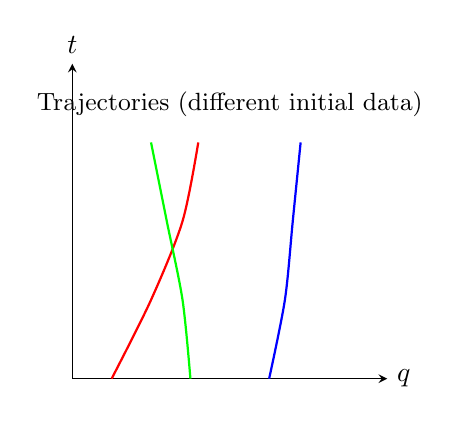
\begin{tikzpicture}[>=stealth,scale=1]
      % Axes
      \draw[->] (0,0) -- (4,0) node[right] {$q$};
      \draw[->] (0,0) -- (0,4) node[above] {$t$};
      % Sample trajectories
      \draw[thick,red,smooth]   plot coordinates {(0.5,0) (1,1) (1.4,2) (1.6,3)};
      \draw[thick,green,smooth] plot coordinates {(1.5,0) (1.4,1) (1.2,2) (1.0,3)};
      \draw[thick,blue,smooth]  plot coordinates {(2.5,0) (2.7,1) (2.8,2) (2.9,3)};
      \node[above] at (2,3.2) {\small Trajectories (different initial data)};
    \end{tikzpicture}
    \caption{Hamilton’s trajectories}
  \end{subfigure}
  \quad
  \begin{subfigure}[b]{0.45\textwidth}
    \centering
    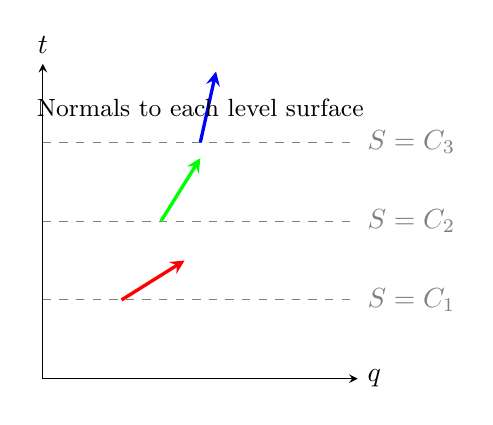
\begin{tikzpicture}[>=stealth,scale=1]
      % Axes
      \draw[->] (0,0) -- (4,0) node[right] {$q$};
      \draw[->] (0,0) -- (0,4) node[above] {$t$};
      % Level‐surface contours of S
      \draw[dashed,gray] (0,1) -- (4,1) node[right] {$S=C_1$};
      \draw[dashed,gray] (0,2) -- (4,2) node[right] {$S=C_2$};
      \draw[dashed,gray] (0,3) -- (4,3) node[right] {$S=C_3$};
      % Normals (∂S/∂q) in matching colors, different directions:
      \draw[->,red,very thick]   (1,1)   -- ++(0.8,0.5);   % ~32°
      \draw[->,green,very thick] (1.5,2) -- ++(0.5,0.8);   % ~58°
      \draw[->,blue,very thick]  (2,3)   -- ++(0.2,0.9);   % ~78°
      \node[above] at (2,3.2) {\small Normals to each level surface};
    \end{tikzpicture}
    \caption{Jacobi’s level surfaces}
  \end{subfigure}
  \caption{%
  Left: individual solution curves (red, green, blue) in the \((q,t)\) plane.  
  Right: contour lines of a single function \(S(q,t)\), with normals (colored arrows) pointing in different directions—each normal reproduces one of the trajectories by \(p_i=\partial S/\partial q_i\).}
\end{figure}
  
  







\subsection{From Flow to Landscape: Mechanics Reimagined}

Jacobi’s insight wasn’t just technical; it was deeply conceptual.  He revealed that the motion of a system—previously seen as a flow of points in phase space—could equally be viewed as the geometry of a single “landscape” defined by

\[
S(q_1,\dots,q_n,t) \;=\;\text{constant}.
\]

In this picture, each possible motion follows the contours of \(S\), much like a hiker tracing a contour line on a topographic map or a light ray moving normal to an optical wavefront.

Instead of integrating Hamilton’s first‐order equations one trajectory at a time, one need only understand the shape of the surface \(S\).  The “steepest ascent” (or descent) of \(S\)—its gradient directions—then reproduces every dynamical path:

\[
p_i \;=\;\frac{\partial S}{\partial q_i}.
\]

\begin{itemize}
  \item \textbf{A single surface for all motion.}  One solves a single PDE for \(S(q,t)\) and immediately obtains the entire family of trajectories as its level‐set contours.
  \item \textbf{Optics and mechanics unite.}  Similar to how Fermat’s wavefronts guide light rays, Jacobi’s action surfaces guide mechanical paths.
  \item \textbf{Geometry supplanting computation.}  Dynamics becomes an exercise in understanding and deforming a landscape, rather than repeatedly integrating equations.  Canonical transformations then appear as mappings that reshape this landscape into simpler forms.
\end{itemize}

In this way, Jacobi elevated mechanics from the calculus of trajectories to the geometry of hypersurfaces:  
the problem of motion became the problem of understanding a single, all‐encompassing geometric object whose contours contain every solution at once.  

In short: 

\begin{itemize}
  \item In Lagrange, we minimized action.  
  \item In Hamilton, we traced flows.  
  \item In Jacobi, we found the surfaces those flows glide along.
\end{itemize}


\begin{figure}[H]
  \centering
  \begin{subfigure}[b]{0.45\textwidth}
    \centering
    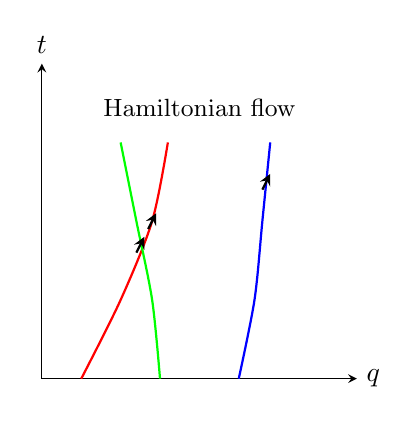
\begin{tikzpicture}[>=stealth,scale=1]
      % Axes
      \draw[->] (0,0) -- (4,0) node[right] {$q$};
      \draw[->] (0,0) -- (0,4) node[above] {$t$};
      % Sample trajectories
      \draw[thick,red,smooth]   plot coordinates {(0.5,0) (1,1) (1.4,2) (1.6,3)};
      \draw[thick,green,smooth] plot coordinates {(1.5,0) (1.4,1) (1.2,2) (1.0,3)};
      \draw[thick,blue,smooth]  plot coordinates {(2.5,0) (2.7,1) (2.8,2) (2.9,3)};
      % Direction arrows along flows
      \foreach \x/\y in {1.2/1.6,1.35/1.9,2.8/2.4} {
        \draw[->,thick] (\x,\y) -- ++(0.1,0.2);
      }
      \node[above] at (2,3.2) {\small Hamiltonian flow};
    \end{tikzpicture}
    \caption{Mechanics as flow}
  \end{subfigure}
  \quad
  \begin{subfigure}[b]{0.45\textwidth}
    \centering
    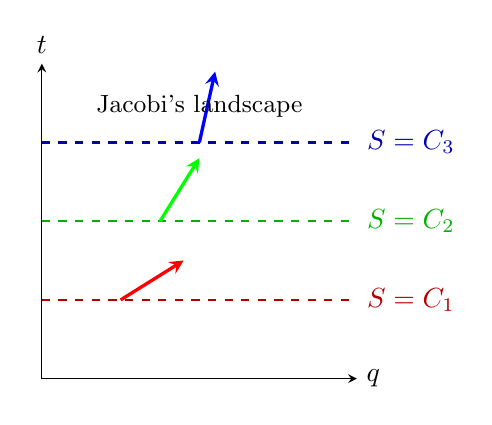
\begin{tikzpicture}[>=stealth,scale=1]
      % Axes
      \draw[->] (0,0) -- (4,0) node[right] {$q$};
      \draw[->] (0,0) -- (0,4) node[above] {$t$};
      % Colored contour lines for S = C1, C2, C3
      \draw[red!70!black,dashed,thick]   (0,1) -- (4,1) node[right] {$S=C_1$};
      \draw[green!70!black,dashed,thick] (0,2) -- (4,2) node[right] {$S=C_2$};
      \draw[blue!70!black,dashed,thick]  (0,3) -- (4,3) node[right] {$S=C_3$};
      % Normals (gradients) in matching colors, different directions
      \draw[->,red,very thick]   (1,1)   -- ++(0.8,0.5);
      \draw[->,green,very thick] (1.5,2) -- ++(0.5,0.8);
      \draw[->,blue,very thick]  (2,3)   -- ++(0.2,0.9);
      \node[above] at (2,3.2) {\small Jacobi’s landscape};
    \end{tikzpicture}
    \caption{Mechanics as geometry}
  \end{subfigure}
  \caption{%
  (\emph{Left}) Hamiltonian picture: each colored curve is a distinct trajectory in \((q,t)\).  
  (\emph{Right}) Jacobi’s picture: the three colored dashed lines are contour lines \(S=C_i\), and the normals (colored arrows) to each contour reproduce exactly the same three trajectories via 
  \(\displaystyle p_i=\partial S/\partial q_i\).}
\end{figure}


In the left panel, three distinct curves (red, green, blue) show individual solutions \(q(t)\) of Hamilton’s equations 
for different initial conditions—each trajectory must be obtained by integrating the ODEs separately.  In the right 
panel, three colored contour lines \(S=C_1,\,C_2,\,C_3\) of a single function \(S(q,t)\) replace those multiple curves.  
The bold arrows (of matching colors) are the normals \(\nabla S\) to each contour, and their directions coincide 
with the trajectories on the left.  Thus, instead of computing many solution curves, Jacobi’s formulation encodes 
all possible motions in the geometry of one surface and its level-set normals.




  
  
  





\subsection{Setting the Stage for a Geometry of Functions}

Jacobi’s great innovation was to show that mechanics need not be built around forces acting on points, but rather around the \emph{shape of a function} \(S(q,t)\).  Instead of asking “What push moves the particle from here to there?”, we ask “What does the landscape of \(S\) look like, and how do its slopes guide motion?”

In this view, dynamics becomes the study of contours, gradients and curvature of a single object:

  A one‐dimensional example: take 
  \[
    S(x) = \tfrac12\,k\,x^2.
  \]
  Its graph is a parabola.  The slope \(dS/dx = kx\) vanishes at \(x=0\), and “motion” along level‐sets carries a fictitious particle toward the minimum—just as a spring pulls a mass back to equilibrium.

  \begin{figure}[H]
    \centering
    \begin{tikzpicture}[>=stealth,scale=1]
      % Axes
      \draw[->] (-3,0) -- (3,0) node[right] {$x$};
      \draw[->] (0,0) -- (0,4) node[above] {$S(x)$};
    
      % Parabola S(x)=½ k x² with k=1
      \draw[thick,blue,domain=-2.5:2.5,smooth,samples=200]
        plot (\x,{0.5*\x*\x});
    
      % Equilibrium (minimum)
      \filldraw[black] (0,0) circle (1.5pt) node[below left] {equilibrium};
    
      % Level‐set “contours” at S=1 and S=2
      \foreach \y in {1,2} {
        \pgfmathsetmacro\xval{sqrt(2*\y)}
        \draw[dashed,gray] (-\xval,\y) -- (\xval,\y) node[right] {$S=\y$};
        \filldraw[gray] (\xval,\y) circle (1.5pt);
        \filldraw[gray] (-\xval,\y) circle (1.5pt);
      }
    
      % Sample point x0 = 1.5
      \def\xo{1.5}
      \coordinate (P) at (\xo,{0.5*\xo*\xo});
      \filldraw[red] (P) circle (2pt) node[above right] {$(x_0,S(x_0))$};
    
      % Tangent line at P: slope = x0
      \draw[red,dashed] ($(P)+(-1,-\xo)$) -- ($(P)+(1,\xo)$)
        node[right] {tangent};
    
      % Gradient arrow (negative slope)
      \draw[->,green!60!black,thick] (P) -- ++(-1,-\xo)
        node[midway,below left] {$-\dfrac{dS}{dx}$};
    
      % Label derivative formula
      \node at (2.5,3.5) {$\displaystyle \frac{dS}{dx}=k\,x$};
    
    \end{tikzpicture}
    \caption{%
    The graph of $S(x)=\tfrac12kx^2$ (here $k=1$) with horizontal “contour” lines (level‐sets) at $S=1$ and $S=2$.  
    Each dashed line marks a level‐set of $S$, intersecting the parabola in two symmetric points.  
    At a sample point $x_0$, the tangent (dashed red) and the negative gradient (green arrow) illustrate how the landscape of $S$ guides motion along its level‐sets.}
  \end{figure}
    




  A two‐dimensional potential surface:
  \[
    S(x,y) = \tfrac12\,m(\dot x^2 + \dot y^2) - V(x,y).
  \]
  One can picture \(S\) as a hilly terrain where valleys correspond to low action.  The particle’s path follows “ridges” and “valleys” of \(S\), determined purely by its shape.

  \begin{figure}[H]
    \centering
    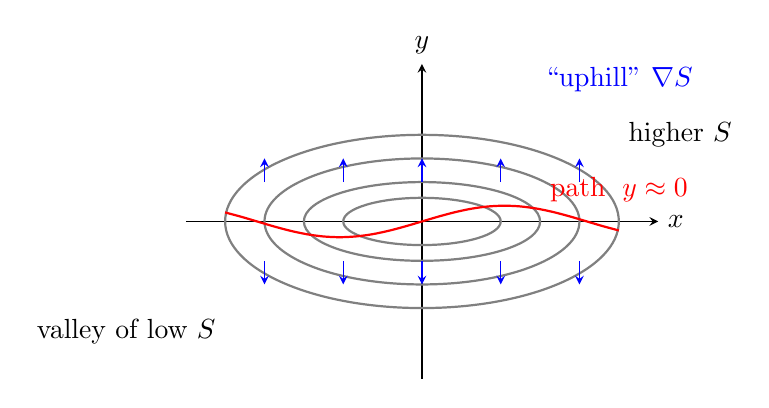
\begin{tikzpicture}[>=stealth,scale=1]
      % Axes
      \draw[->] (-3,0) -- (3,0) node[right] {$x$};
      \draw[->] (0,-2) -- (0,2) node[above] {$y$};
    
      % Contour lines of S(x,y)
      \foreach \a/\b in {1/0.3,1.5/0.5,2/0.8,2.5/1.1}{
        \draw[gray,thick] (0,0) ellipse (\a cm and \b cm);
      }
      \node at (2.5,1.1) [right] {higher $S$};
    
      % Valley floor path
      \draw[red,thick,smooth,domain=-2.5:2.5] plot(\x,{0.2*sin(1.5*\x r)});
      \node[red] at (2.5,0.4) {path \(\;y\approx0\)};
    
      % Gradient arrows (pointing uphill)
      \foreach \x in {-2,-1,0,1,2}{
        \draw[blue,->] (\x,0.5) -- ++(0,0.3);
        \draw[blue,->] (\x,-0.5) -- ++(0,-0.3);
      }
      \node[blue] at (2.5,1.8) {“uphill” $\nabla S$};
    
      % Valley label
      \node at (-2.5,-1.4) [left] {valley of low $S$};
    
    \end{tikzpicture}
    \caption{Contour plot of the two‐dimensional action surface 
    \(\displaystyle S(x,y)=\tfrac12\,m(\dot x^2+\dot y^2)-V(x,y)\). 
    Gray ellipses are level‐sets of \(S\), valleys near \(y=0\) correspond to low action, and the red curve shows the particle’s path following the valley floor.  Blue arrows indicate the gradient \(\nabla S\) pointing “uphill.”}
  \end{figure}


  Optical analogy: Fermat’s wavefronts are level‐sets of the optical path length \(S(\mathbf{r})\).  Light rays then travel normal to these wavefronts.  In mechanics, trajectories likewise run “downhill” in the action landscape.

  Gradient flow vs.\ force laws:  In the traditional Newtonian picture, acceleration comes from a force \(F = -dV/dq\).  In the Jacobi picture, that same acceleration emerges from the curvature of \(S\)—from how rapidly the slopes \(dS/dq\) change in space.

\textbf{Why a geometry of functions?}

\begin{itemize}
  \item It unifies all trajectories: one surface \(S\) contains every possible motion as a contour.
  \item It reveals hidden symmetries: flat directions in \(S\) (zero curvature) correspond to conserved quantities.
  \item It connects to modern ideas: in quantum mechanics, the action \(S\) becomes the phase of a wavefunction, and its level‐sets the wavefronts.
\end{itemize}

By thinking of physics as the study of a single landscape rather than countless individual paths, Jacobi—and those who followed—opened the door to seeing dynamics itself as geometry.  




\subsection{Kepler’s Second Law from Jacobi’s Action Surfaces}

In the Hamilton–Jacobi approach one finds a principal function of the form
\[
S(r,\theta,t) \;=\; W_r(r)\;+\;p_\theta\,\theta \;-\;E\,t,
\]
so that
\[
p_\theta \;=\;\frac{\partial S}{\partial \theta}
\;=\;\text{constant}.
\]
Just as in the purely Hamiltonian picture, this constant conjugate momentum means the phase‐space motion in the \((\theta,p_\theta)\) plane is a horizontal line.  The “area” under that line between angles \(\theta_1\) and \(\theta_2\) is
\[
\int_{\theta_1}^{\theta_2} p_\theta\,d\theta
\;=\;
p_\theta\,(\theta_2-\theta_1),
\]
and, since symplectic area conservation now follows from the geometry of Jacobi’s single action surface, equal increments \(\Delta\theta\) in equal times correspond to equal physical areas \(\Delta A\) in the real orbit:
\[
\Delta A \;=\;\tfrac{1}{2m}\,p_\theta\,\Delta\theta.
\]
Thus Kepler’s Second Law arises directly from the uniform “twist” of the action surface in the \(\theta\) direction.

\begin{figure}[H]
\centering
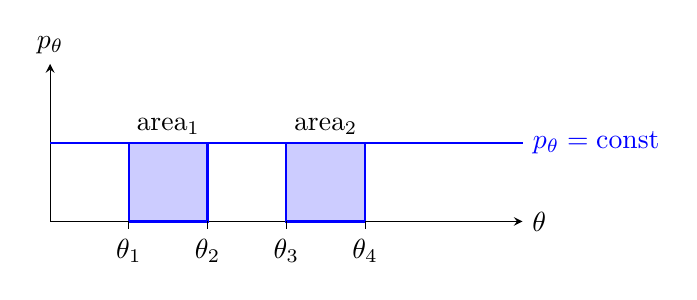
\begin{tikzpicture}[>=stealth, scale=1]
  % Axes
  \draw[->] (0,0) -- (6,0) node[right] {$\theta$};
  \draw[->] (0,0) -- (0,2) node[above] {$p_\theta$};
  % Constant momentum line
  \draw[thick,blue] (0,1) -- (6,1) node[right] {$p_\theta=\mathrm{const}$};
  % Shaded equal-area rectangles
  \fill[blue!20] (1,0) rectangle (2,1);
  \fill[blue!20] (3,0) rectangle (4,1);
  \draw[blue,thick] (1,0) rectangle (2,1) (3,0) rectangle (4,1);
  % Angle ticks and labels
  \foreach \x/\lab in {1/\theta_1,2/\theta_2,3/\theta_3,4/\theta_4} {
    \draw (\x,0) -- (\x,-0.1) node[below] {\(\lab\)};
  }
  % Area labels
  \node at (1.5,1.2) {area$_1$};
  \node at (3.5,1.2) {area$_2$};
\end{tikzpicture}
\caption{In the \((\theta,p_\theta)\) plane, Jacobi’s action surfaces produce the horizontal line \(p_\theta=\mathrm{const}\).  Equal angular intervals \(\Delta\theta\) under this line sweep out equal “action‐space” rectangles \(p_\theta\,\Delta\theta\), which correspond to equal physical areas in the orbit by \(\Delta A = \tfrac{1}{2m}\,p_\theta\,\Delta\theta\).}
\end{figure}

\subsection{Hamiltonian vs.\ Jacobi in the \((\theta,p_\theta)\) Plane}

Although both the Hamiltonian and Hamilton–Jacobi formalisms lead to a constant‐momentum line in the \((\theta,p_\theta)\) plane, the interpretations differ:

\begin{itemize}
  \item \textbf{Hamiltonian:}  \(p_\theta = m\,r^2\dot\theta\) is conserved by the flow; the line is a phase‐space trajectory.
  \item \textbf{Jacobi:}  \(p_\theta = \partial S/\partial \theta\) is constant because the action surface \(S(r,\theta)\) is “twisted” uniformly in \(\theta\); the line is a level‐set gradient of \(S\).
\end{itemize}




\begin{figure}[H]
\centering
\begin{subfigure}[b]{0.7\textwidth}
  \centering
  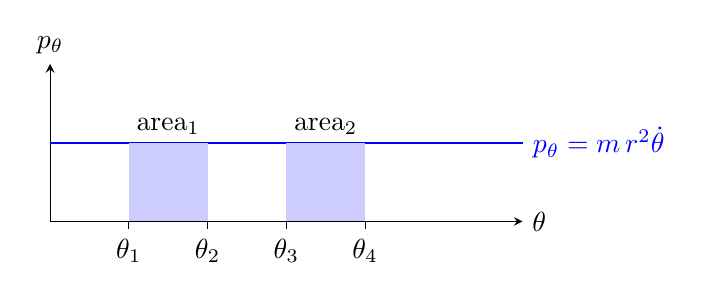
\begin{tikzpicture}[>=stealth, scale=1]
    % Axes
    \draw[->] (0,0) -- (6,0) node[right] {$\theta$};
    \draw[->] (0,0) -- (0,2) node[above] {$p_\theta$};
    % Hamiltonian constant momentum
    \draw[thick,blue] (0,1) -- (6,1) node[right] {$p_\theta = m\,r^2\dot\theta$};
    % Shaded rectangles
    \fill[blue!20] (1,0) rectangle (2,1);
    \fill[blue!20] (3,0) rectangle (4,1);
    % Labels
    \node at (1.5,1.2) {area$_1$};
    \node at (3.5,1.2) {area$_2$};
    % Ticks
    \foreach \x/\lab in {1/\theta_1,2/\theta_2,3/\theta_3,4/\theta_4} {
      \draw (\x,0) -- (\x,-0.1) node[below] {\(\lab\)};
    }
  \end{tikzpicture}
  \caption{Hamiltonian phase space}
\end{subfigure}

\vspace{1em}

\begin{subfigure}[b]{0.7\textwidth}
  \centering
  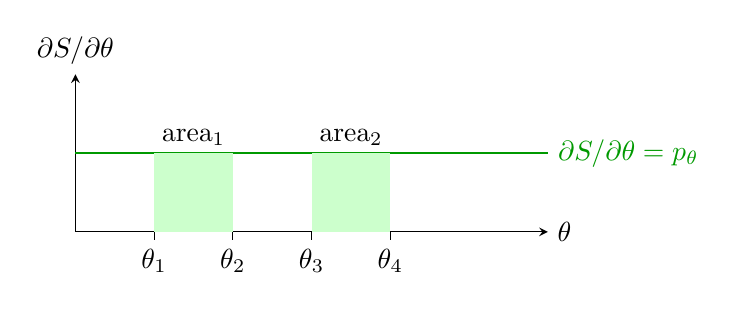
\begin{tikzpicture}[>=stealth, scale=1]
    % Axes
    \draw[->] (0,0) -- (6,0) node[right] {$\theta$};
    \draw[->] (0,0) -- (0,2) node[above] {$\partial S/\partial \theta$};
    % Jacobi constant gradient
    \draw[thick,green!60!black] (0,1) -- (6,1) node[right] {\(\partial S/\partial \theta = p_\theta\)};
    % Shaded rectangles
    \fill[green!20] (1,0) rectangle (2,1);
    \fill[green!20] (3,0) rectangle (4,1);
    % Labels
    \node at (1.5,1.2) {area$_1$};
    \node at (3.5,1.2) {area$_2$};
    % Ticks
    \foreach \x/\lab in {1/\theta_1,2/\theta_2,3/\theta_3,4/\theta_4} {
      \draw (\x,0) -- (\x,-0.1) node[below] {\(\lab\)};
    }
  \end{tikzpicture}
  \caption{Jacobi action‐surface gradient}
\end{subfigure}

\caption{Comparison of the constant‐momentum interpretation: (top) Hamiltonian phase‐space flow, (bottom) Jacobi’s uniform “twist” of the action surface.  In both pictures equal angular intervals \(\Delta\theta\) sweep out equal areas, but the underlying geometry differs.}
\end{figure}

\begin{figure}[H]
  \centering
  % 1) Cartesian orbit
  \subcaptionbox{Physical ellipse in $(x,y)$ plane\label{fig:kepler-cartesian}}{%
    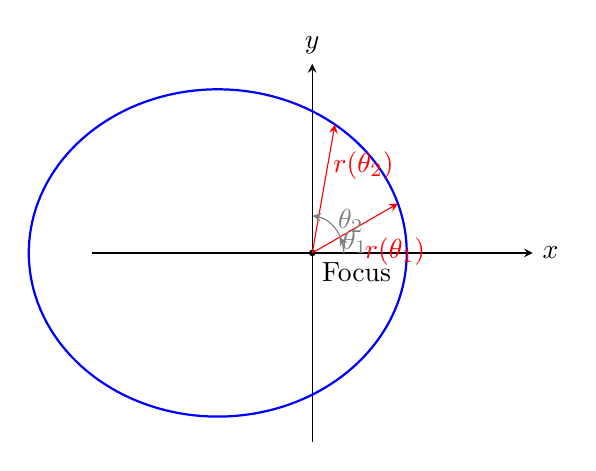
\begin{tikzpicture}[>=stealth,scale=0.8]
      % Axes
      \draw[->] (-3.5,0) -- (3.5,0) node[right] {$x$};
      \draw[->] (0,-3) -- (0,3) node[above] {$y$};
      % Ellipse (a=3, e=0.5)
      \draw[thick,blue,domain=0:360,smooth,samples=200]
        plot ({(2.25/(1+0.5*cos(\x)))*cos(\x)},
             {(2.25/(1+0.5*cos(\x)))*sin(\x)});
      % Focus
      \fill (0,0) circle (1.5pt) node[below right] {Focus};
      % Sample radii at θ1=30°, θ2=80°
      \def\thA{30} \def\thB{80}
      \pgfmathsetmacro\rA{2.25/(1+0.5*cos(\thA))}
      \pgfmathsetmacro\rB{2.25/(1+0.5*cos(\thB))}
      \coordinate (A) at ({\rA*cos(\thA)},{\rA*sin(\thA)});
      \coordinate (B) at ({\rB*cos(\thB)},{\rB*sin(\thB)});
      \draw[red,->] (0,0) -- (A) node[midway,below right] {$r(\theta_1)$};
      \draw[red,->] (0,0) -- (B) node[midway,above right] {$r(\theta_2)$};
      % Angle markers
      \draw[gray,->] (0.5,0) arc[start angle=0,end angle=\thA,radius=0.5];
      \node[gray] at ({0.7*cos(\thA/2)},{0.7*sin(\thA/2)}) {$\theta_1$};
      \draw[gray,->] (0.5,0) arc[start angle=0,end angle=\thB,radius=0.6];
      \node[gray] at ({0.8*cos(\thB/2)},{0.8*sin(\thB/2)}) {$\theta_2$};
    \end{tikzpicture}
  }
  
  \vspace{1em}
  
  % 2) Hamiltonian phase space
  \subcaptionbox{Hamiltonian $(\theta,p_\theta)$ plane\label{fig:kepler-ham}}{%
    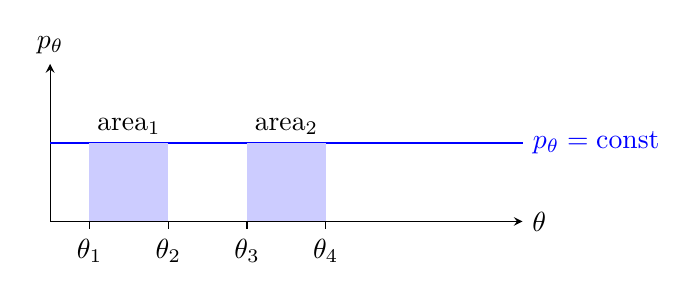
\begin{tikzpicture}[>=stealth,scale=1]
      % Axes
      \draw[->] (0,0) -- (6,0) node[right] {$\theta$};
      \draw[->] (0,0) -- (0,2) node[above] {$p_\theta$};
      % Constant momentum line
      \draw[thick,blue] (0,1) -- (6,1) node[right] {$p_\theta=\mathrm{const}$};
      % Shaded equal-area intervals matching θ1,θ2
      \fill[blue!20] (0.5,0) rectangle (1.5,1);
      \fill[blue!20] (2.5,0) rectangle (3.5,1);
      % Area labels
      \node at (1,1.2) {area$_1$};
      \node at (3,1.2) {area$_2$};
      % Tick marks
      \draw (0.5,0) -- (0.5,-0.1) node[below] {$\theta_1$};
      \draw (1.5,0) -- (1.5,-0.1) node[below] {$\theta_2$};
      \draw (2.5,0) -- (2.5,-0.1) node[below] {$\theta_3$};
      \draw (3.5,0) -- (3.5,-0.1) node[below] {$\theta_4$};
    \end{tikzpicture}
  }
  
  \vspace{1em}
  
  % 3) Jacobi action-surface gradient
  \subcaptionbox{Jacobi $(\theta,\partial S/\partial\theta)$ plane\label{fig:kepler-jac}}{%
    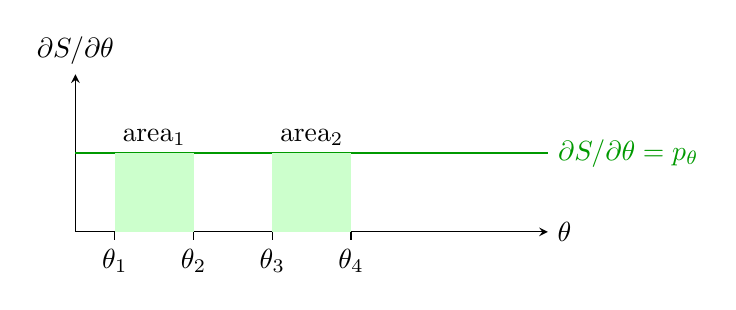
\begin{tikzpicture}[>=stealth,scale=1]
      % Axes
      \draw[->] (0,0) -- (6,0) node[right] {$\theta$};
      \draw[->] (0,0) -- (0,2) node[above] {$\partial S/\partial\theta$};
      % Constant gradient line
      \draw[thick,green!60!black] (0,1) -- (6,1) node[right] {$\partial S/\partial\theta = p_\theta$};
      % Shaded equal-area intervals
      \fill[green!20] (0.5,0) rectangle (1.5,1);
      \fill[green!20] (2.5,0) rectangle (3.5,1);
      % Area labels
      \node at (1,1.2) {area$_1$};
      \node at (3,1.2) {area$_2$};
      % Tick marks
      \draw (0.5,0) -- (0.5,-0.1) node[below] {$\theta_1$};
      \draw (1.5,0) -- (1.5,-0.1) node[below] {$\theta_2$};
      \draw (2.5,0) -- (2.5,-0.1) node[below] {$\theta_3$};
      \draw (3.5,0) -- (3.5,-0.1) node[below] {$\theta_4$};
    \end{tikzpicture}
  }
  
  \caption{%
  (\subref{fig:kepler-cartesian}) The actual elliptical orbit in Cartesian coordinates, showing radius vectors at $\theta_1,\theta_2$.  
  (\subref{fig:kepler-ham}) The Hamiltonian phase‐space interpretation: equal angular slices $\Delta\theta$ sweep out equal phase‐space areas under $p_\theta=\mathrm{const}$.  
  (\subref{fig:kepler-jac}) The Jacobi action‐surface gradient view: equal $\Delta\theta$ slices under the constant $\partial S/\partial\theta$ line also produce equal areas, reflecting the same areal law via the action surface.}
  \end{figure}
  